% include the figures path relative to the master file
\graphicspath{ {./content/method/figures/} }

\section{Data}\label{sec:data}
In order to compare different methodologies, the first requirement is access to a common pull of images.
Despite the fact that lack of public data is a common claim within the medical image community~\cite{giger2008anniversary}, the community developing methodologies for \gls{sdoct} imagery has public data available~\cite{DUKEDATA_a,DUKEDATA_b}, mainly gathered at \emph{Duke University}.
However this data has deficiencies that makes it unsuitable for our problem.
Venhuizen\,\emph{et. al.} test using a large public dataset of $384$ \gls{oct} annotated volumes of \gls{amd}\,\emph{vs.\,normal} cases.
Despite the interest of testing against a large dataset, our goal remains not to detect \gls{amd} but to study the detection of \gls{dme}.
Srinivasan\,\textit{et~al.}~\cite{Srinivasan2014} also test using a public dataset from \emph{Duke Univeristy}, this time containing \gls{amd}, \gls{dme} and \emph{normal} volumes.
However, the volumes of this dataset have been manipulated using pre-processing, realignment, cropping, etc. and there original data is not available making the dataset unsuited for our purposes.

Therefore, we use the \gls{seri} dataset~\cite{SERIDATA} to conduct this study (see fig.\,\ref{fig:bbdd}).
This dataset was acquired by the \gls{seri}, using CIRRUS TM (Carl Zeiss Meditec, Inc., Dublin, CA) \gls{sdoct} device.
The dataset consists of 32 \gls{oct} volumes (16 \gls{dme} and 16 normal cases).
Each volume contains 128 B-scan with resolution of 512 $\times$ 1024 pixels.  All \gls{sdoct} images are read and assessed by trained graders and identified as normal or \gls{dme} cases based on evaluation of retinal thickening, hard exudates, intraretinal cystoid space formation and subretinal fluid.

\begin{figure}
  \centering{
    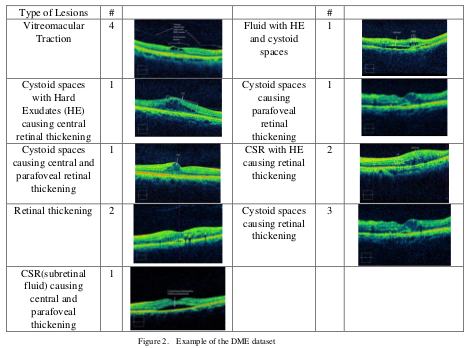
\includegraphics[width=1\linewidth]{bbdd}}
    \caption{\gls{seri} dataset description.}
  \label{fig:bbdd}
\end{figure}
